% Options for packages loaded elsewhere
\PassOptionsToPackage{unicode}{hyperref}
\PassOptionsToPackage{hyphens}{url}
\PassOptionsToPackage{dvipsnames,svgnames,x11names}{xcolor}
%
\documentclass[
  letterpaper,
  DIV=11,
  numbers=noendperiod]{scrartcl}

\usepackage{amsmath,amssymb}
\usepackage{iftex}
\ifPDFTeX
  \usepackage[T1]{fontenc}
  \usepackage[utf8]{inputenc}
  \usepackage{textcomp} % provide euro and other symbols
\else % if luatex or xetex
  \usepackage{unicode-math}
  \defaultfontfeatures{Scale=MatchLowercase}
  \defaultfontfeatures[\rmfamily]{Ligatures=TeX,Scale=1}
\fi
\usepackage{lmodern}
\ifPDFTeX\else  
    % xetex/luatex font selection
\fi
% Use upquote if available, for straight quotes in verbatim environments
\IfFileExists{upquote.sty}{\usepackage{upquote}}{}
\IfFileExists{microtype.sty}{% use microtype if available
  \usepackage[]{microtype}
  \UseMicrotypeSet[protrusion]{basicmath} % disable protrusion for tt fonts
}{}
\makeatletter
\@ifundefined{KOMAClassName}{% if non-KOMA class
  \IfFileExists{parskip.sty}{%
    \usepackage{parskip}
  }{% else
    \setlength{\parindent}{0pt}
    \setlength{\parskip}{6pt plus 2pt minus 1pt}}
}{% if KOMA class
  \KOMAoptions{parskip=half}}
\makeatother
\usepackage{xcolor}
\setlength{\emergencystretch}{3em} % prevent overfull lines
\setcounter{secnumdepth}{5}
% Make \paragraph and \subparagraph free-standing
\makeatletter
\ifx\paragraph\undefined\else
  \let\oldparagraph\paragraph
  \renewcommand{\paragraph}{
    \@ifstar
      \xxxParagraphStar
      \xxxParagraphNoStar
  }
  \newcommand{\xxxParagraphStar}[1]{\oldparagraph*{#1}\mbox{}}
  \newcommand{\xxxParagraphNoStar}[1]{\oldparagraph{#1}\mbox{}}
\fi
\ifx\subparagraph\undefined\else
  \let\oldsubparagraph\subparagraph
  \renewcommand{\subparagraph}{
    \@ifstar
      \xxxSubParagraphStar
      \xxxSubParagraphNoStar
  }
  \newcommand{\xxxSubParagraphStar}[1]{\oldsubparagraph*{#1}\mbox{}}
  \newcommand{\xxxSubParagraphNoStar}[1]{\oldsubparagraph{#1}\mbox{}}
\fi
\makeatother


\providecommand{\tightlist}{%
  \setlength{\itemsep}{0pt}\setlength{\parskip}{0pt}}\usepackage{longtable,booktabs,array}
\usepackage{calc} % for calculating minipage widths
% Correct order of tables after \paragraph or \subparagraph
\usepackage{etoolbox}
\makeatletter
\patchcmd\longtable{\par}{\if@noskipsec\mbox{}\fi\par}{}{}
\makeatother
% Allow footnotes in longtable head/foot
\IfFileExists{footnotehyper.sty}{\usepackage{footnotehyper}}{\usepackage{footnote}}
\makesavenoteenv{longtable}
\usepackage{graphicx}
\makeatletter
\def\maxwidth{\ifdim\Gin@nat@width>\linewidth\linewidth\else\Gin@nat@width\fi}
\def\maxheight{\ifdim\Gin@nat@height>\textheight\textheight\else\Gin@nat@height\fi}
\makeatother
% Scale images if necessary, so that they will not overflow the page
% margins by default, and it is still possible to overwrite the defaults
% using explicit options in \includegraphics[width, height, ...]{}
\setkeys{Gin}{width=\maxwidth,height=\maxheight,keepaspectratio}
% Set default figure placement to htbp
\makeatletter
\def\fps@figure{htbp}
\makeatother

\usepackage{booktabs}
\usepackage{longtable}
\usepackage{array}
\usepackage{multirow}
\usepackage{wrapfig}
\usepackage{float}
\usepackage{colortbl}
\usepackage{pdflscape}
\usepackage{tabu}
\usepackage{threeparttable}
\usepackage{threeparttablex}
\usepackage[normalem]{ulem}
\usepackage{makecell}
\usepackage{xcolor}
\KOMAoption{captions}{tableheading}
\makeatletter
\@ifpackageloaded{caption}{}{\usepackage{caption}}
\AtBeginDocument{%
\ifdefined\contentsname
  \renewcommand*\contentsname{Table of contents}
\else
  \newcommand\contentsname{Table of contents}
\fi
\ifdefined\listfigurename
  \renewcommand*\listfigurename{List of Figures}
\else
  \newcommand\listfigurename{List of Figures}
\fi
\ifdefined\listtablename
  \renewcommand*\listtablename{List of Tables}
\else
  \newcommand\listtablename{List of Tables}
\fi
\ifdefined\figurename
  \renewcommand*\figurename{Figure}
\else
  \newcommand\figurename{Figure}
\fi
\ifdefined\tablename
  \renewcommand*\tablename{Table}
\else
  \newcommand\tablename{Table}
\fi
}
\@ifpackageloaded{float}{}{\usepackage{float}}
\floatstyle{ruled}
\@ifundefined{c@chapter}{\newfloat{codelisting}{h}{lop}}{\newfloat{codelisting}{h}{lop}[chapter]}
\floatname{codelisting}{Listing}
\newcommand*\listoflistings{\listof{codelisting}{List of Listings}}
\makeatother
\makeatletter
\makeatother
\makeatletter
\@ifpackageloaded{caption}{}{\usepackage{caption}}
\@ifpackageloaded{subcaption}{}{\usepackage{subcaption}}
\makeatother

\ifLuaTeX
\usepackage[bidi=basic]{babel}
\else
\usepackage[bidi=default]{babel}
\fi
\babelprovide[main,import]{english}
% get rid of language-specific shorthands (see #6817):
\let\LanguageShortHands\languageshorthands
\def\languageshorthands#1{}
\ifLuaTeX
  \usepackage{selnolig}  % disable illegal ligatures
\fi
\usepackage{bookmark}

\IfFileExists{xurl.sty}{\usepackage{xurl}}{} % add URL line breaks if available
\urlstyle{same} % disable monospaced font for URLs
\hypersetup{
  pdftitle={Rscience},
  pdfauthor={Rscience},
  pdflang={en},
  colorlinks=true,
  linkcolor={blue},
  filecolor={Maroon},
  citecolor={Blue},
  urlcolor={Blue},
  pdfcreator={LaTeX via pandoc}}


\title{Rscience}
\author{Rscience}
\date{2026-01-06}

\begin{document}
\maketitle

\renewcommand*\contentsname{Table of contents}
{
\hypersetup{linkcolor=}
\setcounter{tocdepth}{2}
\tableofcontents
}

\newpage

\section{Anova Outpus}\label{anova-outpus}

\subsection{Anova Table}\label{anova-table}

\begin{longtable}[]{@{}
  >{\raggedright\arraybackslash}p{(\columnwidth - 12\tabcolsep) * \real{0.1429}}
  >{\raggedright\arraybackslash}p{(\columnwidth - 12\tabcolsep) * \real{0.3000}}
  >{\raggedleft\arraybackslash}p{(\columnwidth - 12\tabcolsep) * \real{0.0429}}
  >{\raggedleft\arraybackslash}p{(\columnwidth - 12\tabcolsep) * \real{0.1429}}
  >{\raggedleft\arraybackslash}p{(\columnwidth - 12\tabcolsep) * \real{0.1429}}
  >{\raggedleft\arraybackslash}p{(\columnwidth - 12\tabcolsep) * \real{0.1286}}
  >{\raggedleft\arraybackslash}p{(\columnwidth - 12\tabcolsep) * \real{0.1000}}@{}}
\toprule\noalign{}
\begin{minipage}[b]{\linewidth}\raggedright
\end{minipage} & \begin{minipage}[b]{\linewidth}\raggedright
Sources of Variation
\end{minipage} & \begin{minipage}[b]{\linewidth}\raggedleft
Df
\end{minipage} & \begin{minipage}[b]{\linewidth}\raggedleft
Sum Sq
\end{minipage} & \begin{minipage}[b]{\linewidth}\raggedleft
Mean Sq
\end{minipage} & \begin{minipage}[b]{\linewidth}\raggedleft
F value
\end{minipage} & \begin{minipage}[b]{\linewidth}\raggedleft
Pr(\textgreater F)
\end{minipage} \\
\midrule\noalign{}
\endhead
\bottomrule\noalign{}
\endlastfoot
cyl & Factor & 2 & 824.7846 & 412.39229 & 39.69752 & 0 \\
Residuals & Error & 29 & 301.2626 & 10.38837 & NA & NA \\
Total & Total & 31 & 1126.0472 & 36.32410 & NA & NA \\
\end{longtable}

\subsection{Tukey Table and Plot}\label{tukey-table-and-plot}

\begin{longtable}[]{@{}rlrl@{}}
\toprule\noalign{}
order & level & mean & group \\
\midrule\noalign{}
\endhead
\bottomrule\noalign{}
\endlastfoot
1 & 4 & 26.66364 & a \\
2 & 6 & 19.74286 & b \\
3 & 8 & 15.10000 & c \\
\end{longtable}

\begin{center}
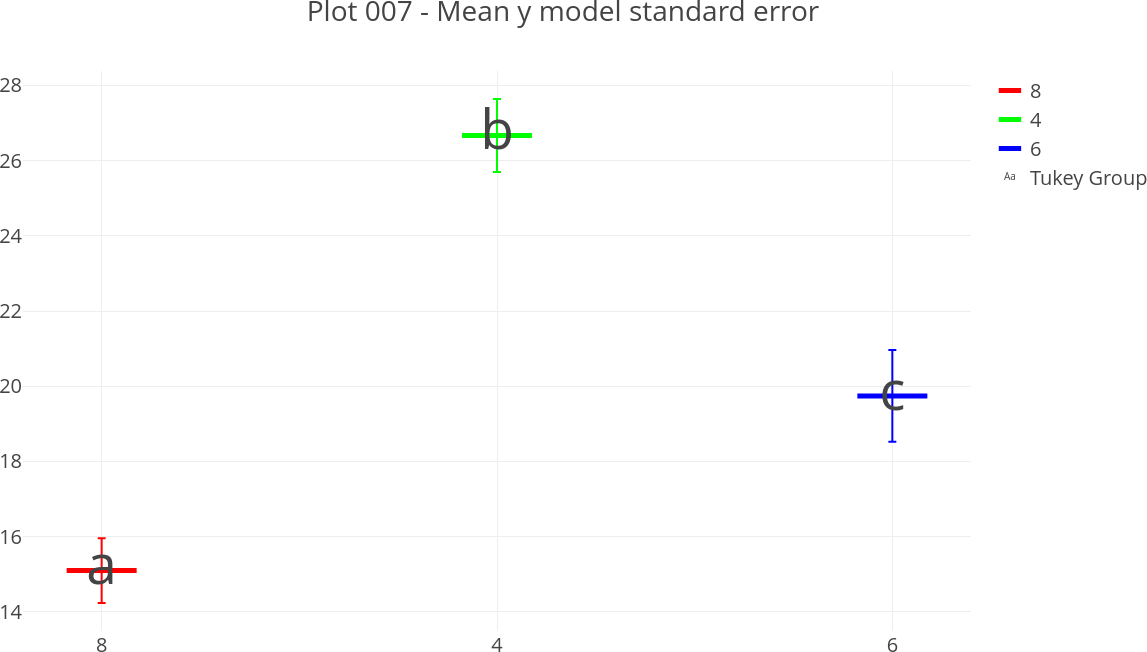
\includegraphics[width=8.33333in,height=5.20833in]{report02_pdf_files/figure-pdf/unnamed-chunk-5-1.png}
\end{center}

\begin{center}
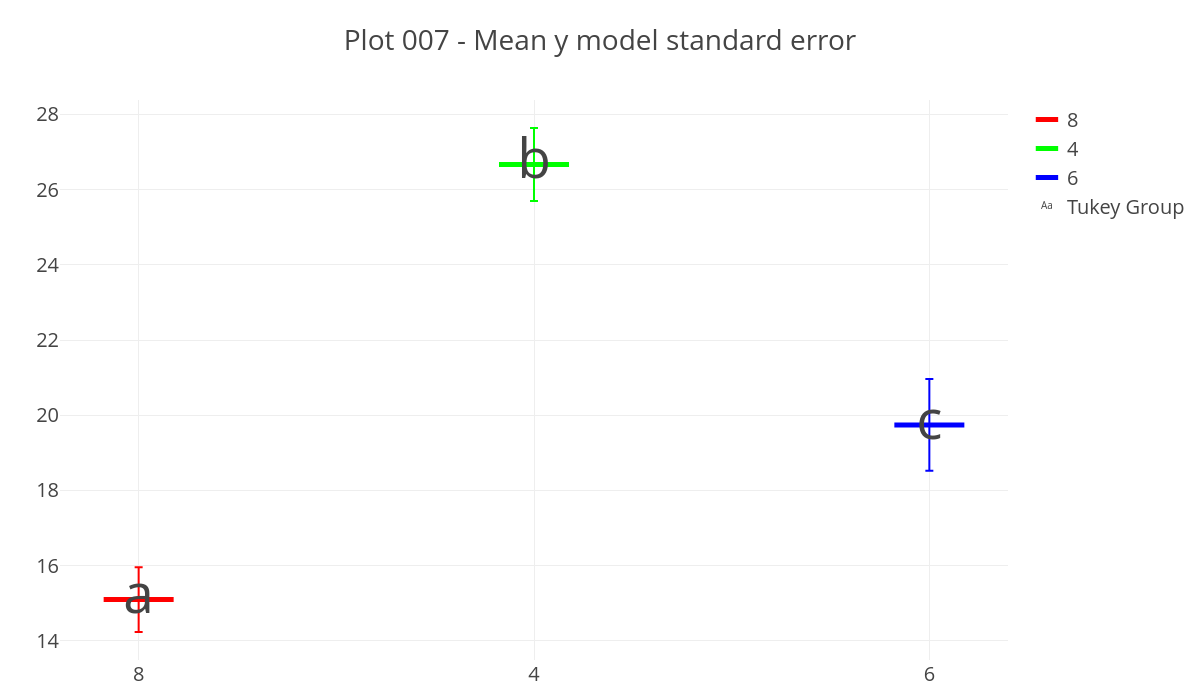
\includegraphics[width=8.33333in,height=5.20833in]{aver.png}
\end{center}

\subsection{Requeriments - Residuals
Normality}\label{requeriments---residuals-normality}

\begin{longtable}[]{@{}llrr@{}}
\toprule\noalign{}
variable & test & statistic(W) & p\_value \\
\midrule\noalign{}
\endhead
\bottomrule\noalign{}
\endlastfoot
residuals & Shapiro-Wilk normality test & 0.9706547 & 0.517665 \\
\end{longtable}

\subsection{Requeriments - Residuals
Homogeneity}\label{requeriments---residuals-homogeneity}

\begin{longtable}[]{@{}
  >{\raggedright\arraybackslash}p{(\columnwidth - 6\tabcolsep) * \real{0.1064}}
  >{\raggedright\arraybackslash}p{(\columnwidth - 6\tabcolsep) * \real{0.4468}}
  >{\raggedleft\arraybackslash}p{(\columnwidth - 6\tabcolsep) * \real{0.3404}}
  >{\raggedleft\arraybackslash}p{(\columnwidth - 6\tabcolsep) * \real{0.1064}}@{}}
\toprule\noalign{}
\begin{minipage}[b]{\linewidth}\raggedright
variable
\end{minipage} & \begin{minipage}[b]{\linewidth}\raggedright
test
\end{minipage} & \begin{minipage}[b]{\linewidth}\raggedleft
statistic(Bartlett's K-squared)
\end{minipage} & \begin{minipage}[b]{\linewidth}\raggedleft
p\_value
\end{minipage} \\
\midrule\noalign{}
\endhead
\bottomrule\noalign{}
\endlastfoot
residuals & Bartlett test of homogeneity of variances & 8.393396 &
0.0150452 \\
\end{longtable}

\newpage

\section{Reporting Level I - Summary
Anova}\label{reporting-level-i---summary-anova}

\subsection{Summary Table}\label{summary-table}

\begin{longtable}[]{@{}
  >{\raggedright\arraybackslash}p{(\columnwidth - 12\tabcolsep) * \real{0.1565}}
  >{\raggedright\arraybackslash}p{(\columnwidth - 12\tabcolsep) * \real{0.1826}}
  >{\raggedright\arraybackslash}p{(\columnwidth - 12\tabcolsep) * \real{0.0870}}
  >{\raggedleft\arraybackslash}p{(\columnwidth - 12\tabcolsep) * \real{0.0870}}
  >{\raggedleft\arraybackslash}p{(\columnwidth - 12\tabcolsep) * \real{0.1043}}
  >{\raggedright\arraybackslash}p{(\columnwidth - 12\tabcolsep) * \real{0.2609}}
  >{\raggedright\arraybackslash}p{(\columnwidth - 12\tabcolsep) * \real{0.1217}}@{}}
\toprule\noalign{}
\begin{minipage}[b]{\linewidth}\raggedright
name
\end{minipage} & \begin{minipage}[b]{\linewidth}\raggedright
test
\end{minipage} & \begin{minipage}[b]{\linewidth}\raggedright
variable
\end{minipage} & \begin{minipage}[b]{\linewidth}\raggedleft
p\_value
\end{minipage} & \begin{minipage}[b]{\linewidth}\raggedleft
alpha\_value
\end{minipage} & \begin{minipage}[b]{\linewidth}\raggedright
Decision
\end{minipage} & \begin{minipage}[b]{\linewidth}\raggedright
Valid
\end{minipage} \\
\midrule\noalign{}
\endhead
\bottomrule\noalign{}
\endlastfoot
Shapiro-Wilk test & Normality & residuals & 0.5176650 & 0.05 & Ho no
rejected & Yes, it is. \\
Bartlett test & Homogeneity & residuals & 0.0150452 & 0.05 & Ho Rejected
& Yes, it is. \\
Anova 1 way & Analysis of Variance & mpg & 0.0000000 & 0.05 & Ho
Rejected & No, is not!!! \\
Tukey & Mean groups & mpg & NA & 0.05 & At least two groups of means. &
No, is not!!! \\
\end{longtable}

\subsection{Phrases}\label{phrases}

The null hypothesis of normal distribution of residuals is not rejected.

The hypothesis of homogeneity of variances (homoscedasticity) is
rejected.

Not all requirements for the model are met.

It is NOT valid to draw conclusions from the ANOVA test.

As the model requirements are not met, the ANOVA and Tukey analyses must
be discarded, irrespective of the statistical values obtained. The
literal and decontextualized interpretation of the ANOVA test and the
Tukey test is detailed below for demonstrative purposes only, but holds
no validity for drawing conclusions from them.

The null hypothesis of the ANOVA test is rejected. There are
statistically significant differences in at least one level of the
factor.

Since the ANOVA null hypothesis is rejected, the use of a multiple
comparison test to accompany the ANOVA test is valid.

The Tukey test is selected as the multiple comparison test for this
script.

The Tukey test indicates that there are at least 2 groups among the
factor levels. The number of groups and their structure must be analyzed
in detail using the Tukey table.

ANOVA indicates that all factor levels are equal, while Tukey has found
at least 2 groups. Tukey is subject to the rejection of the ANOVA
hypothesis. Since the ANOVA null hypothesis is not rejected, the Tukey
test must not be taken into account for decision-making. All factor
levels are equal.

\newpage

\section{Reporting Level II - Decision-Making Process in
ANOVA}\label{reporting-level-ii---decision-making-process-in-anova}

The ANOVA test is specifically performed to make decisions.\\
The decision-making process has a set of sequential steps, in a
particular order.\\
\textbf{Step 01:} Normality Verification\\
\textbf{Step 02:} Homogeneity Verification\\
\textbf{Step 03:} Global Requirements Check\\
\textbf{Step 04:} ANOVA Validation\\
\textbf{Step 05:} ANOVA Interpretation\\
\textbf{Step 06:} Tukey Test Validation\\
\textbf{Step 07:} Tukey Test Interpretation\\
\textbf{Step 08:} ANOVA-Tukey Consistency Analysis\\
\textbf{Step 09:} Final Conclusion

\subsection{\texorpdfstring{\textbf{Step 01:} Normality
Verification}{Step 01: Normality Verification}}\label{step-01-normality-verification}

\begin{longtable}[]{@{}llrr@{}}
\toprule\noalign{}
variable & test & statistic(W) & p\_value \\
\midrule\noalign{}
\endhead
\bottomrule\noalign{}
\endlastfoot
residuals & Shapiro-Wilk normality test & 0.9706547 & 0.517665 \\
\end{longtable}

The p value about normality distibution is 0.517664951040294.\\
Alpha value is 0.05.\\
The p value is equal or mayor than alpha value.\\
The null hypothesis of normal distribution of residuals is not
rejected.\\
Los residuos poseen distribución normal.

\subsection{\texorpdfstring{\textbf{Step 02:} Homogeneity
Verification}{Step 02: Homogeneity Verification}}\label{step-02-homogeneity-verification}

\begin{longtable}[]{@{}
  >{\raggedright\arraybackslash}p{(\columnwidth - 6\tabcolsep) * \real{0.1064}}
  >{\raggedright\arraybackslash}p{(\columnwidth - 6\tabcolsep) * \real{0.4468}}
  >{\raggedleft\arraybackslash}p{(\columnwidth - 6\tabcolsep) * \real{0.3404}}
  >{\raggedleft\arraybackslash}p{(\columnwidth - 6\tabcolsep) * \real{0.1064}}@{}}
\toprule\noalign{}
\begin{minipage}[b]{\linewidth}\raggedright
variable
\end{minipage} & \begin{minipage}[b]{\linewidth}\raggedright
test
\end{minipage} & \begin{minipage}[b]{\linewidth}\raggedleft
statistic(Bartlett's K-squared)
\end{minipage} & \begin{minipage}[b]{\linewidth}\raggedleft
p\_value
\end{minipage} \\
\midrule\noalign{}
\endhead
\bottomrule\noalign{}
\endlastfoot
residuals & Bartlett test of homogeneity of variances & 8.393396 &
0.0150452 \\
\end{longtable}

The p value about homogeneity variances from residuals is
0.0150451770493758.\\
Alpha value is 0.05.\\
The p value is less than alpha value.\\
The null hypothesis of homogeneity of variances from residuals is
rejected.\\
Los residuos son homogeneos.

\subsection{\texorpdfstring{\textbf{Step 03:} Global Requirements
Check}{Step 03: Global Requirements Check}}\label{step-03-global-requirements-check}

Not all requirements for the model are met.

\subsection{\texorpdfstring{\textbf{Step 04:} ANOVA
Validation}{Step 04: ANOVA Validation}}\label{step-04-anova-validation}

It is NOT valid to draw conclusions from the ANOVA test. This dataset
must be analyzed with another statistical tool such as the
Kruskal-Wallis test. If a more sophisticated tool is desired, the
possibility of utilizing generalized linear mixed models, generalized
linear models, generalized linear models, exact distribution linear
models, etc., could be evaluated.

It is NOT valid to draw conclusions from the ANOVA test. As the model
requirements are not met, the ANOVA and Tukey analyses must be
discarded, irrespective of the statistical values obtained. The literal
and decontextualized interpretation of the ANOVA test and the Tukey test
is detailed below for demonstrative purposes only, but holds no validity
for drawing conclusions from them.

\subsection{\texorpdfstring{\textbf{Step 05:} ANOVA
Interpretation}{Step 05: ANOVA Interpretation}}\label{step-05-anova-interpretation}

\begin{longtable}[]{@{}
  >{\raggedright\arraybackslash}p{(\columnwidth - 12\tabcolsep) * \real{0.1429}}
  >{\raggedright\arraybackslash}p{(\columnwidth - 12\tabcolsep) * \real{0.3000}}
  >{\raggedleft\arraybackslash}p{(\columnwidth - 12\tabcolsep) * \real{0.0429}}
  >{\raggedleft\arraybackslash}p{(\columnwidth - 12\tabcolsep) * \real{0.1429}}
  >{\raggedleft\arraybackslash}p{(\columnwidth - 12\tabcolsep) * \real{0.1429}}
  >{\raggedleft\arraybackslash}p{(\columnwidth - 12\tabcolsep) * \real{0.1286}}
  >{\raggedleft\arraybackslash}p{(\columnwidth - 12\tabcolsep) * \real{0.1000}}@{}}
\toprule\noalign{}
\begin{minipage}[b]{\linewidth}\raggedright
\end{minipage} & \begin{minipage}[b]{\linewidth}\raggedright
Sources of Variation
\end{minipage} & \begin{minipage}[b]{\linewidth}\raggedleft
Df
\end{minipage} & \begin{minipage}[b]{\linewidth}\raggedleft
Sum Sq
\end{minipage} & \begin{minipage}[b]{\linewidth}\raggedleft
Mean Sq
\end{minipage} & \begin{minipage}[b]{\linewidth}\raggedleft
F value
\end{minipage} & \begin{minipage}[b]{\linewidth}\raggedleft
Pr(\textgreater F)
\end{minipage} \\
\midrule\noalign{}
\endhead
\bottomrule\noalign{}
\endlastfoot
cyl & Factor & 2 & 824.7846 & 412.39229 & 39.69752 & 0 \\
Residuals & Error & 29 & 301.2626 & 10.38837 & NA & NA \\
Total & Total & 31 & 1126.0472 & 36.32410 & NA & NA \\
\end{longtable}

The p-value for the ANOVA test is 4.97891917440017e-09. The alpha value
is 0.05. The p-value is less than the alpha value. The null hypothesis
of equal means for the ANOVA test is rejected. There are statistically
significant differences in at least one level of the factor. By
rejecting the null hypothesis, the ANOVA test guarantees statistically
significant differences in at least one level of the factor with the
lowest mean and the level of the factor with the highest mean.

\subsection{\texorpdfstring{\textbf{Step 06:} Tukey Test
Validation}{Step 06: Tukey Test Validation}}\label{step-06-tukey-test-validation}

Since the ANOVA null hypothesis is rejected, the use of a multiple
comparison test to accompany the ANOVA test is valid.

The Tukey test is selected as the multiple comparison test for this
script.

\newpage

\subsection{\texorpdfstring{\textbf{Step 07:} Tukey Test
Interpretation}{Step 07: Tukey Test Interpretation}}\label{step-07-tukey-test-interpretation}

The Tukey test details at least 2 statistically different groups. The
group structure detailed by the Tukey test must now be considered in
order to provide a recommendation in your area of work.

\begin{longtable}[]{@{}rlrl@{}}
\toprule\noalign{}
order & level & mean & group \\
\midrule\noalign{}
\endhead
\bottomrule\noalign{}
\endlastfoot
1 & 4 & 26.66364 & a \\
2 & 6 & 19.74286 & b \\
3 & 8 & 15.10000 & c \\
\end{longtable}

\begin{verbatim}
Error in `initialize()`:
! `width` must be a whole number, not the string "100%".
\end{verbatim}

\newpage

\subsection{\texorpdfstring{\textbf{Step 08:} ANOVA-Tukey Consistency
Analysis}{Step 08: ANOVA-Tukey Consistency Analysis}}\label{step-08-anova-tukey-consistency-analysis}

ANOVA indicates that all factor levels are equal, while Tukey has found
at least 2 groups. Tukey is subject to the rejection of the ANOVA
hypothesis. Since the ANOVA null hypothesis is not rejected, the Tukey
test must not be taken into account for decision-making. All factor
levels are equal.

The means of each factor level are detailed with the standard error
derived from the model.\\
The statistical groups from the Tukey test are detailed for each factor
level.

\newpage

\section{Reporting Level III - Automatic Statistic Asesor
(ASA)}\label{reporting-level-iii---automatic-statistic-asesor-asa}

\subsection{General}\label{general}

When not all model requirements (Normality and/or Homogeneity) are met,
the ANOVA analysis is immediately discarded. This invalidation occurs
irrespective of whether the failure is due to non-normality of the
residuals, non-homogeneity, or both requirements. Indistinctly of the
statistical values obtained in the ANOVA test and the Tukey test, it is
NOT valid to draw conclusions of any type; the entire analysis is
completely discarded. An alternative statistical tool or path must be
sought to analyze the data, with the quickest recommended tool being the
Kruskal-Wallis test, although a better analysis may allow for the use of
more robust tools such as Generalized Linear Mixed Models or Exact
Statistics; the alternative statistical path is to perform a
transformation on the response variable and attempt the 1-Factor ANOVA
test again. The statistical options suggested must be verified and
justified for their feasibility of use. Continuing with statistical
interpretations without fulfilling the model's requirements is a serious
error common among those new to statistics, and a common practice among
those lacking the sufficient statistical knowledge to correctly analyze
the reality they intend to study. If, despite all these warnings, you
continue with the analysis, you expose your work to severe criticism
from colleagues, evaluation committees, and publication reviewers.

\subsection{Requeriments}\label{requeriments}

The ANOVA statistical test is based on 3 points for decision-making:
shape, dispersion, and position. The shape is the normal distribution of
the residuals. The dispersion is the homogeneous variances in the
residuals, and the position is the mean of the response variable for one
of the factor levels. By guaranteeing that the shape and dispersion of
the residuals have a certain particular structure, ANOVA manages to test
the position in the response variable. This is why the fulfillment of
normality and homogeneity of variances of the residuals is a
requirement, and only with the simultaneous fulfillment of both
requirements is it valid to make an interpretation of the means. If all
requirements are not met simultaneously, the ANOVA analysis must be
discarded, irrespective of the results it may have yielded. There is no
escape, and you must seek another statistical tool to interpret these
results.

\subsection{Anova}\label{anova}

The model requirements are not met. The ANOVA statistical test has the
indispensable requirement of residual normality and homogeneity of
variances. Both requirements must be met jointly for it to be valid to
draw conclusions about the factor levels. Continuing with the
statistical interpretation without fulfilling all the requirements is a
catastrophic error. The ANOVA model requirements are neither optional
nor can they be assumed. The model requirements are the fundamental
basis upon which the ANOVA test relies to make decisions about the means
of the factor levels. In this case, you must seek another statistical
tool to perform the analysis of your data.

\subsection{Tukey}\label{tukey}

The use of the Tukey test is subject to the validity of the ANOVA model
and the rejection of the ANOVA hypothesis. As the model requirements are
not met, the ANOVA test is not valid, and therefore the Tukey test is
not valid either. The information related to the Tukey test must be
discarded. As detailed before, in this context, continuing with the
statistical interpretation is a serious statistical error that
demonstrates a total lack of statistical criteria for decision-making.




\end{document}
